\section{Evaluation}
\label{sec:evaluation}

\subsection{Dataset}
We collected a dataset comprising of 149 stained tissue images in collaboration with pathologists. The images are taken at a magnification of $10\times$, and are all scaled to a resolution of $1000\times 1000$. Each image in the dataset has been marked as `cancerous' or `non-cancerous' by a pathologist. Some sample images from the dataset are shown in Figure~\ref{fig:TissueImageExample}.

\begin{figure}
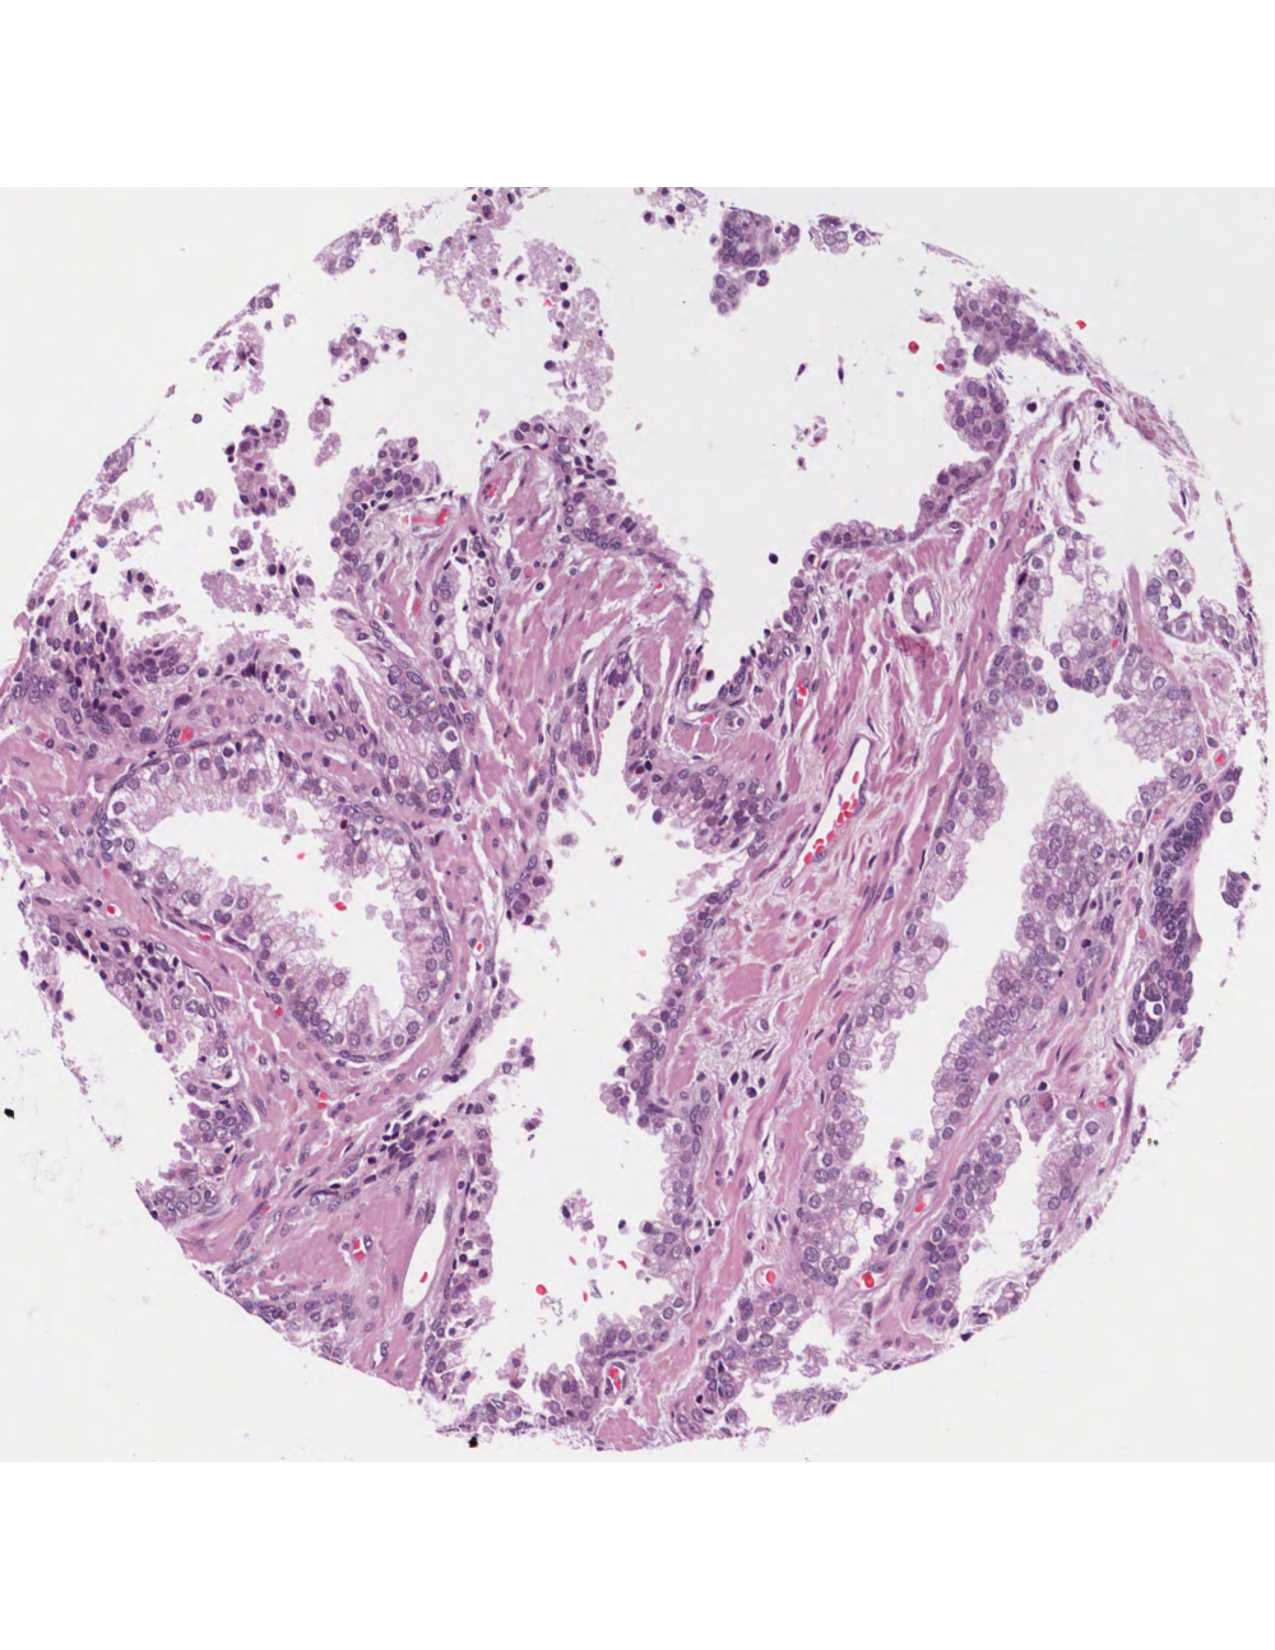
\includegraphics[width=2.0cm]{figs/145_green.pdf}
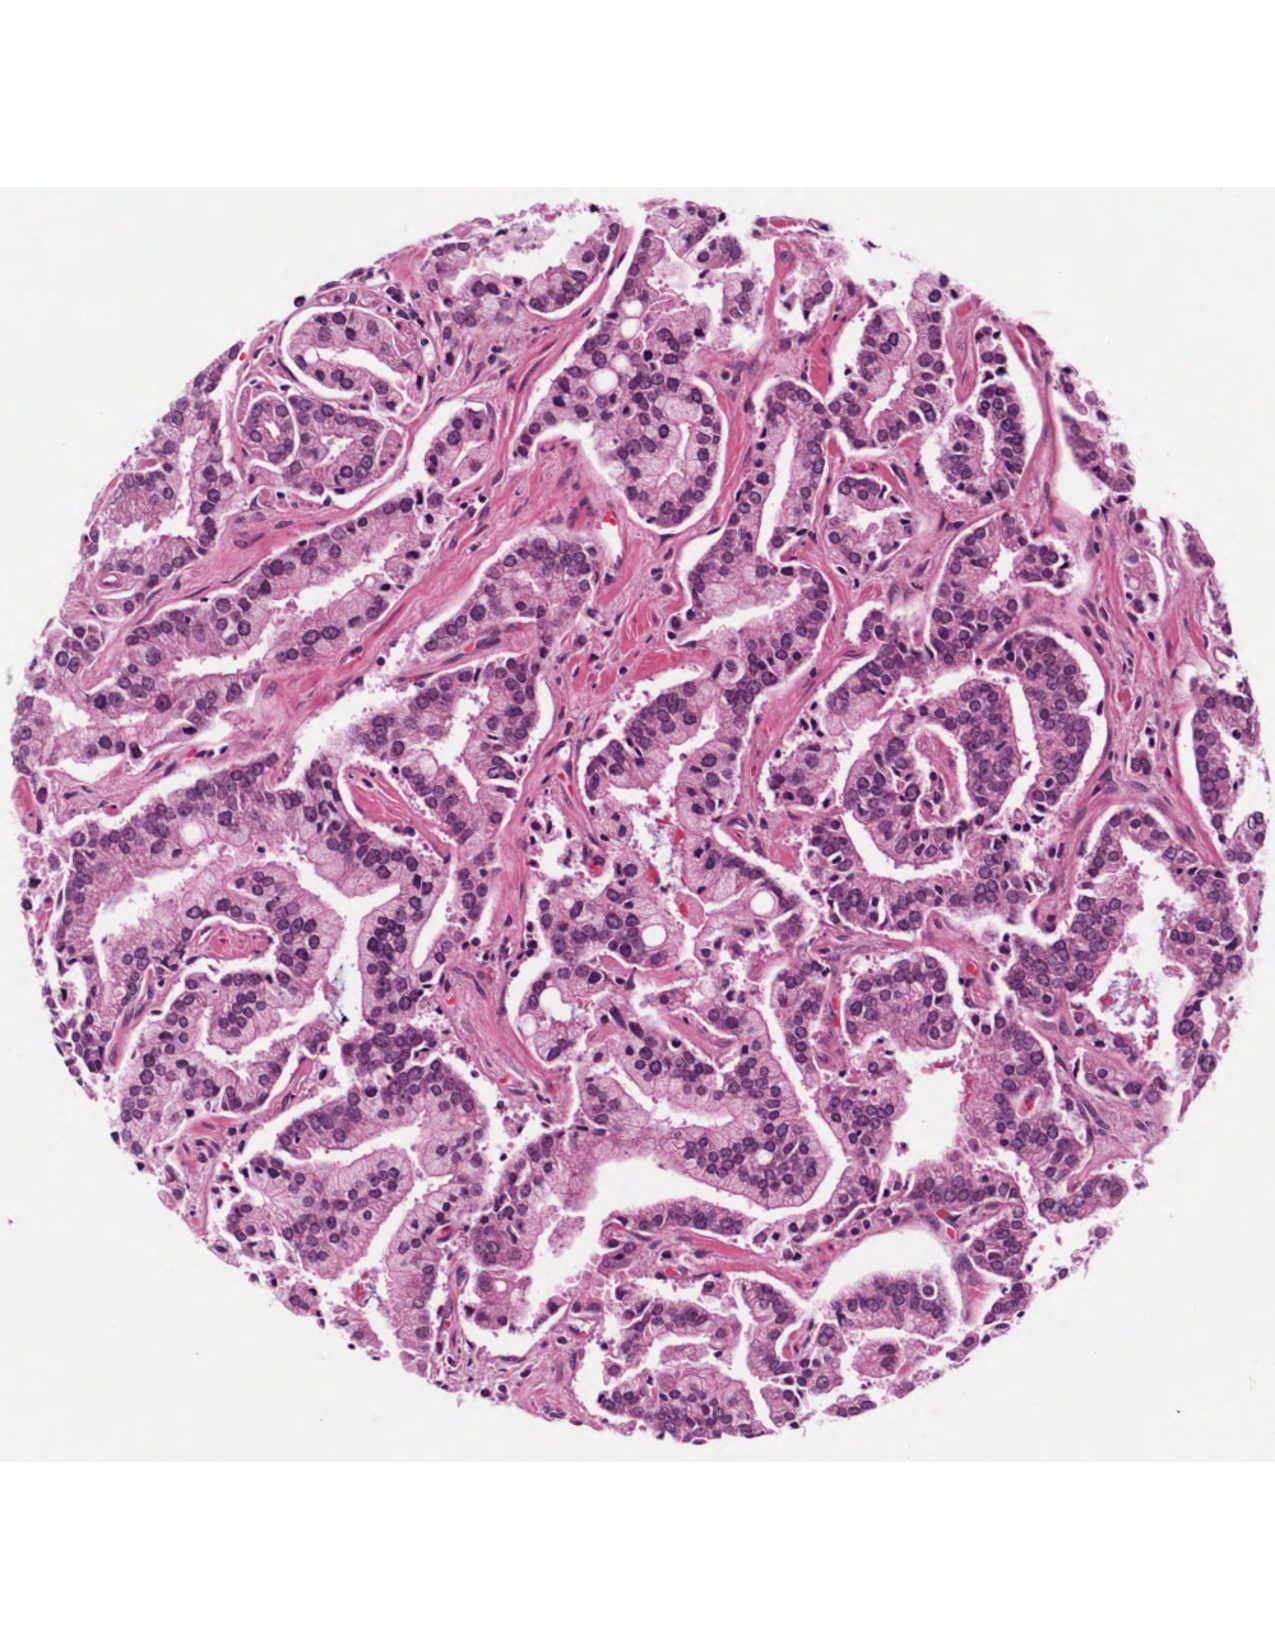
\includegraphics[width=2.0cm]{figs/93_red.pdf}
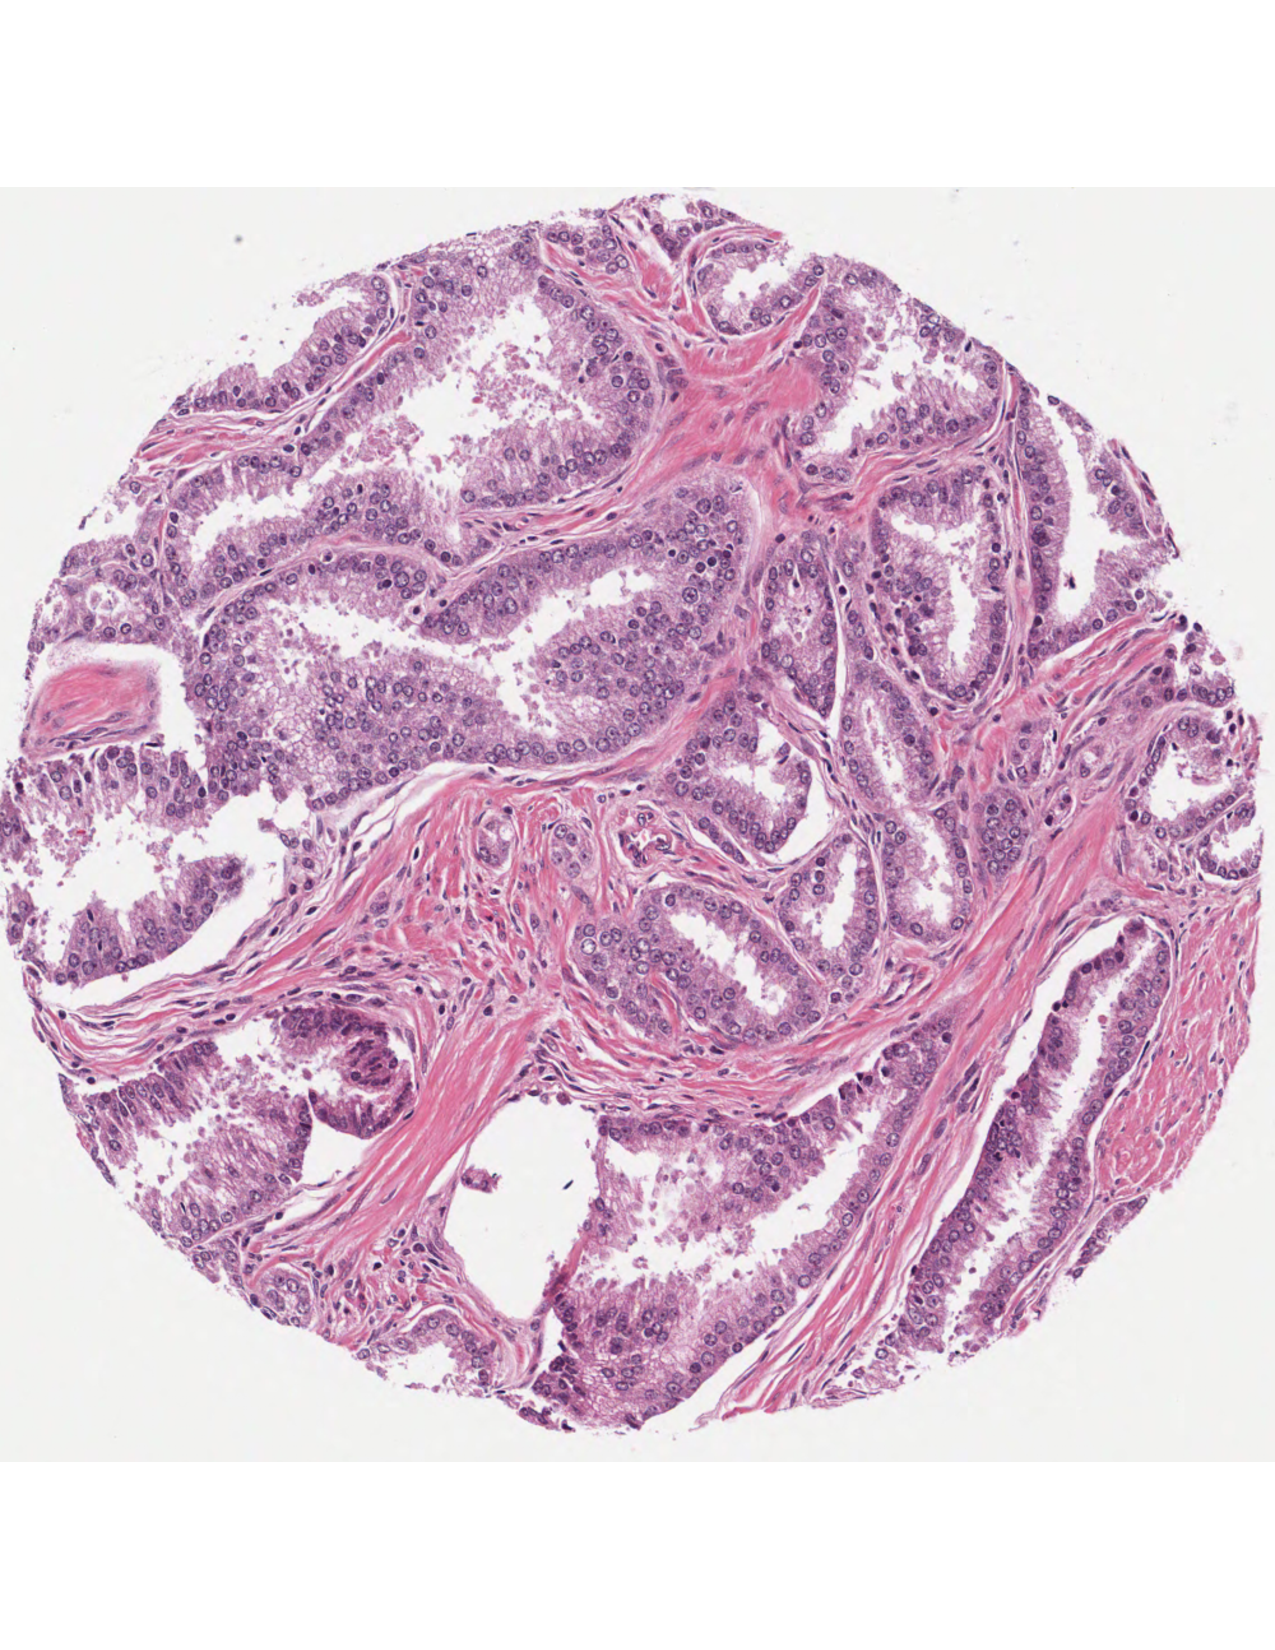
\includegraphics[width=2.0cm]{figs/130_green.pdf}
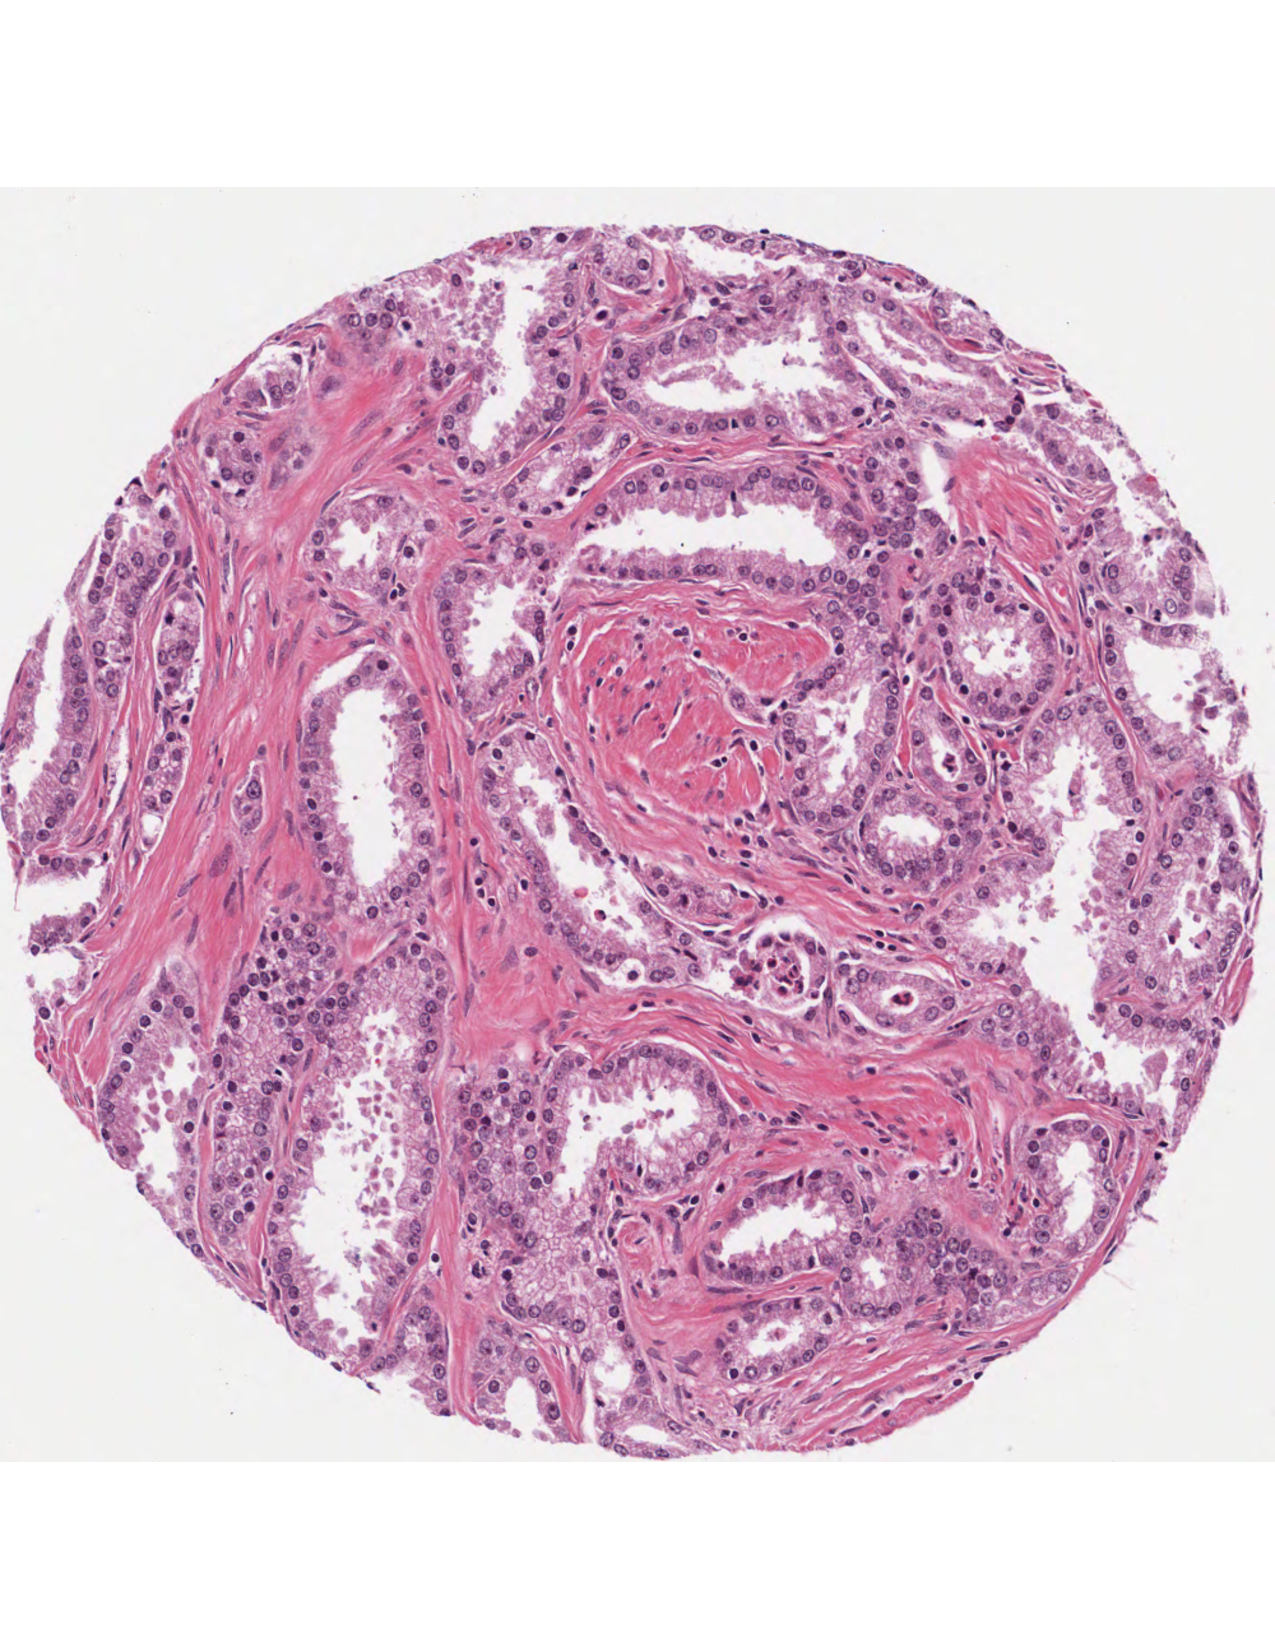
\includegraphics[width=2.0cm]{figs/87_red.pdf}
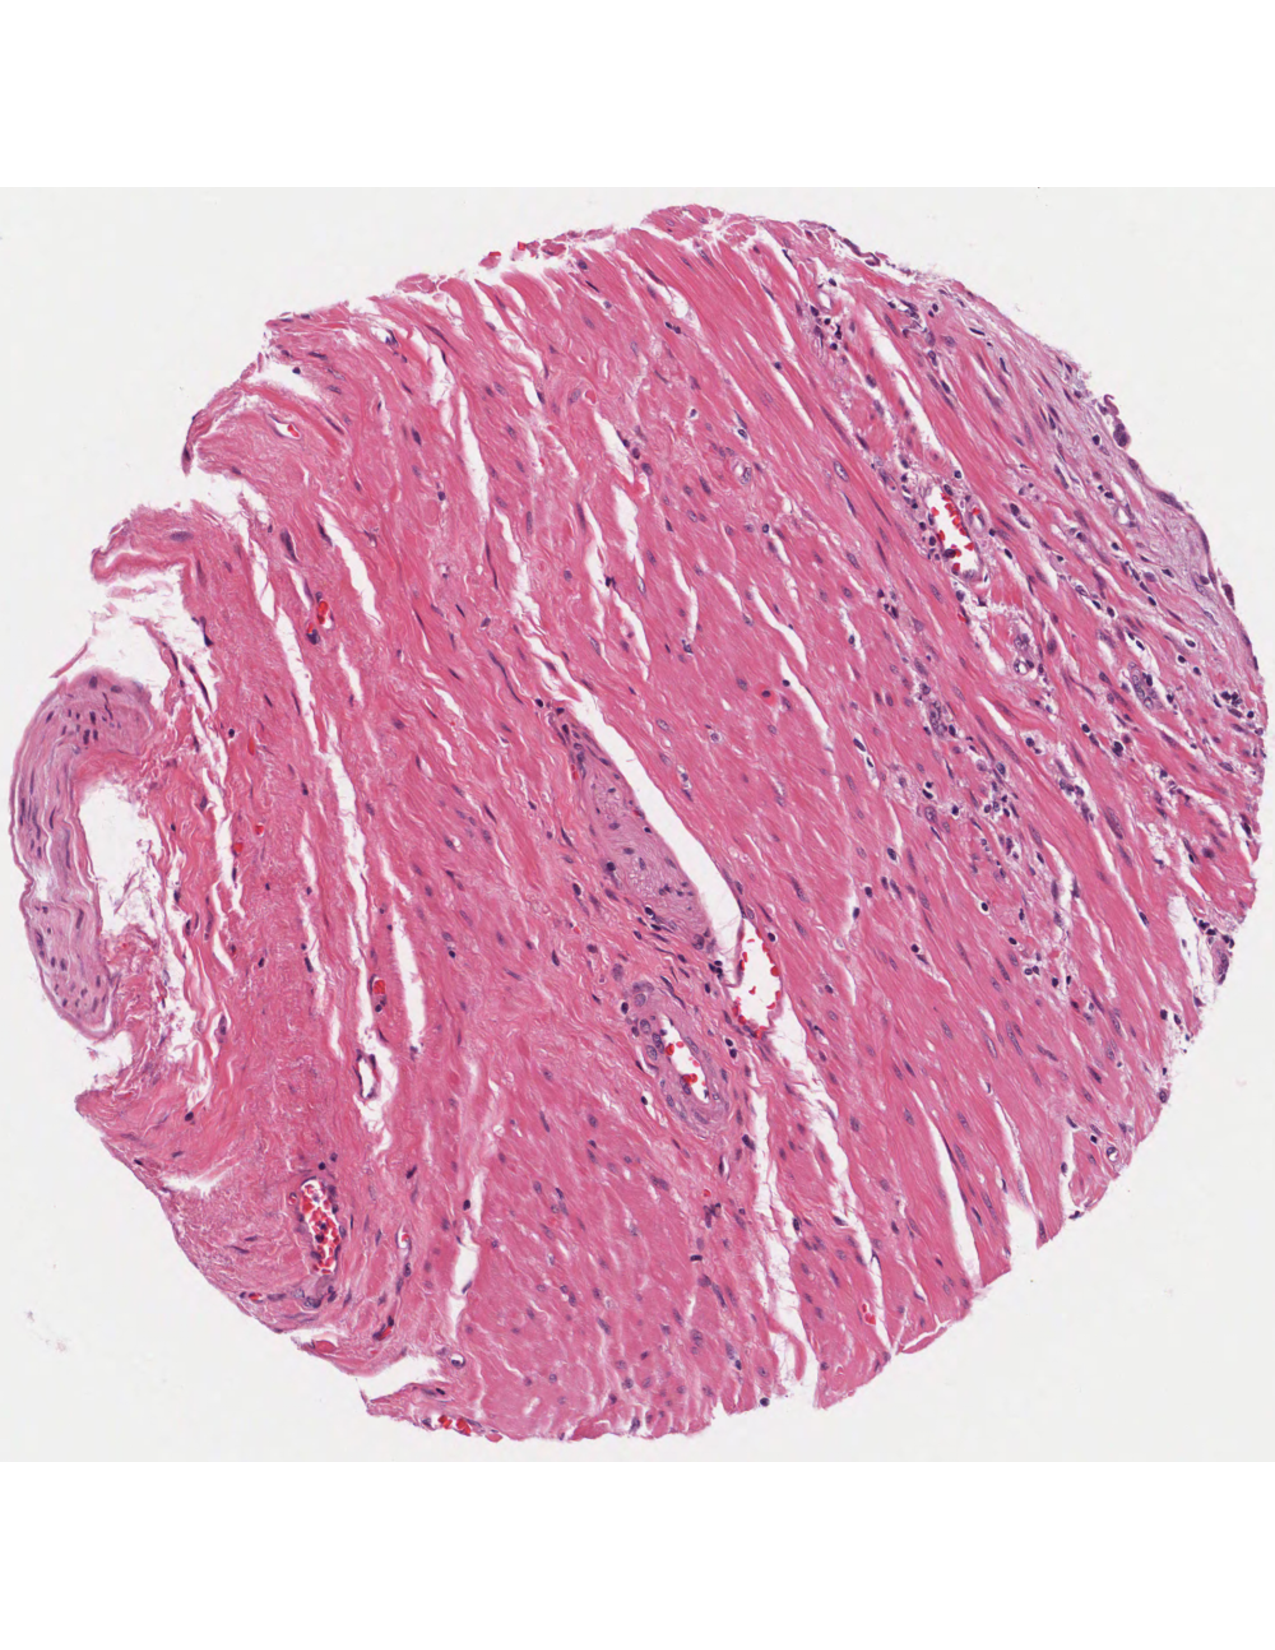
\includegraphics[width=2.0cm]{figs/63_green.pdf}
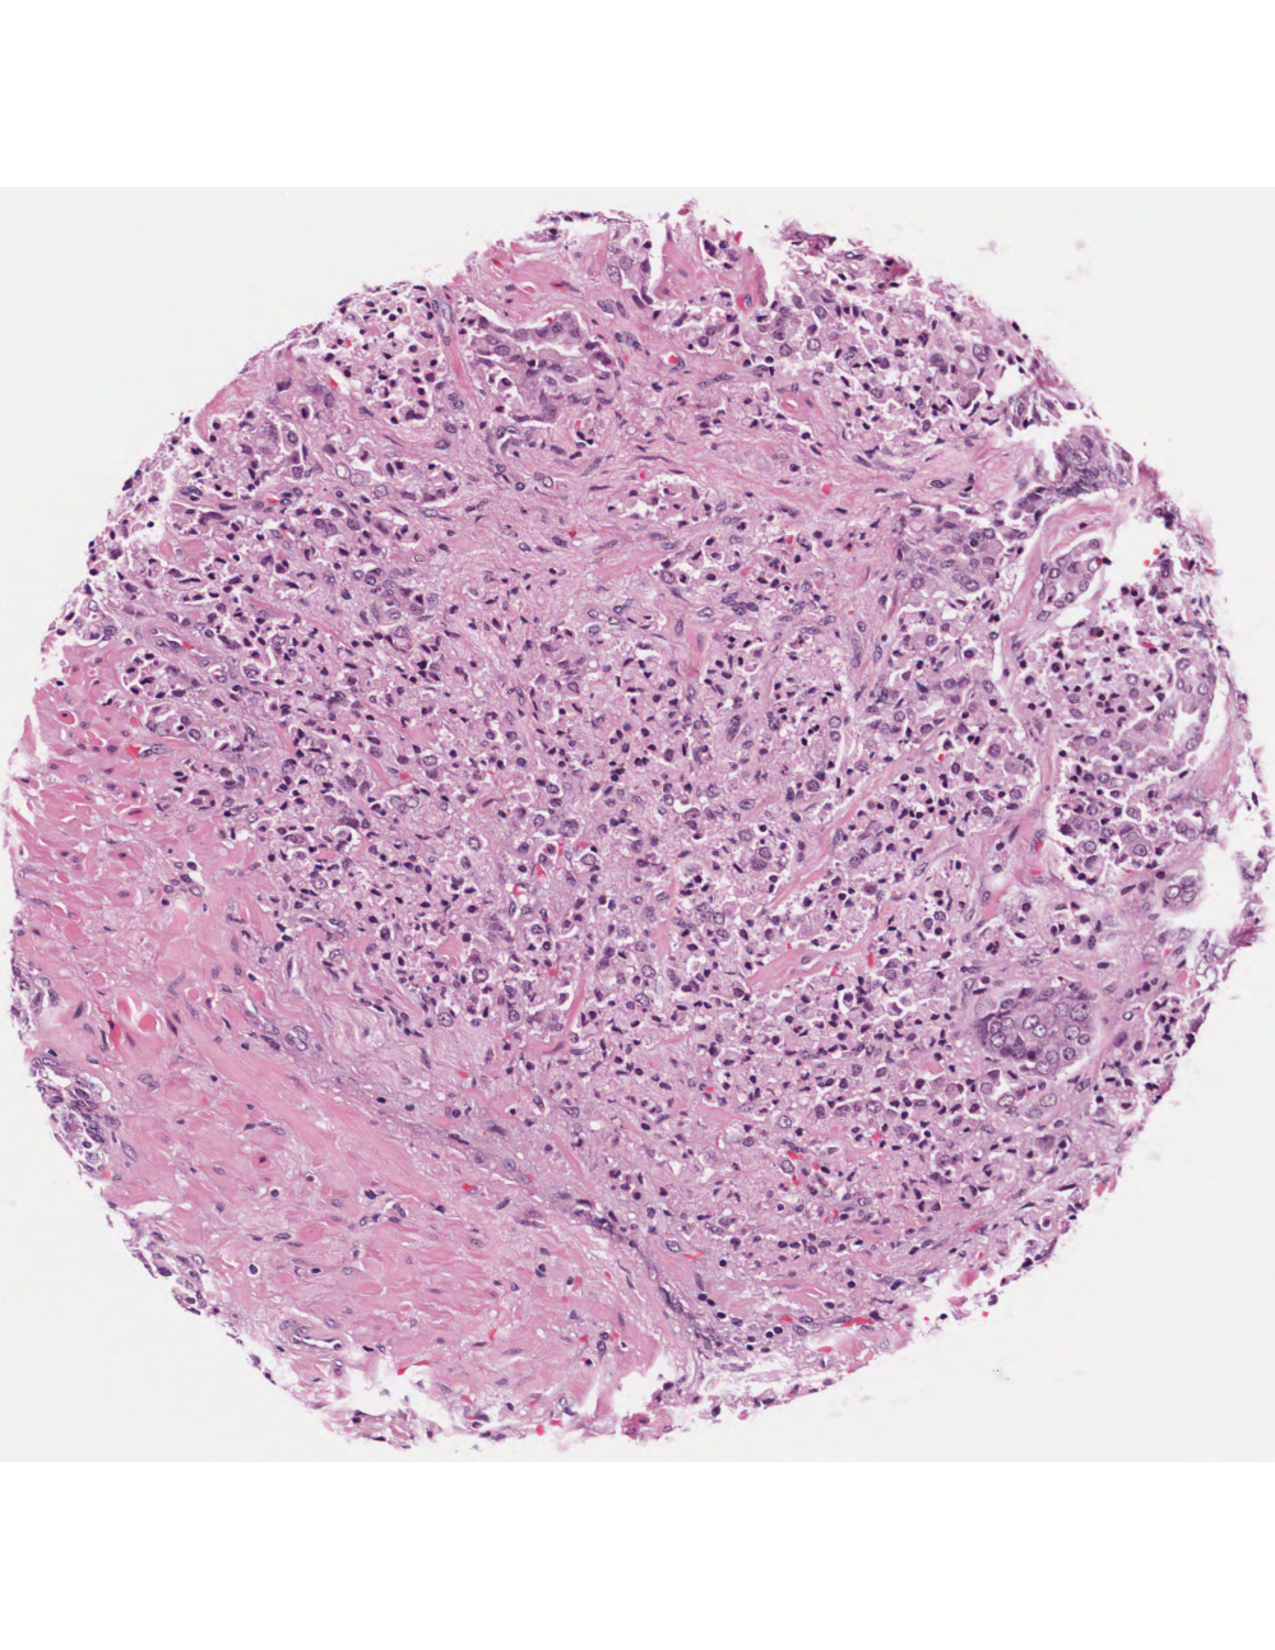
\includegraphics[width=2.0cm]{figs/41_red.pdf}
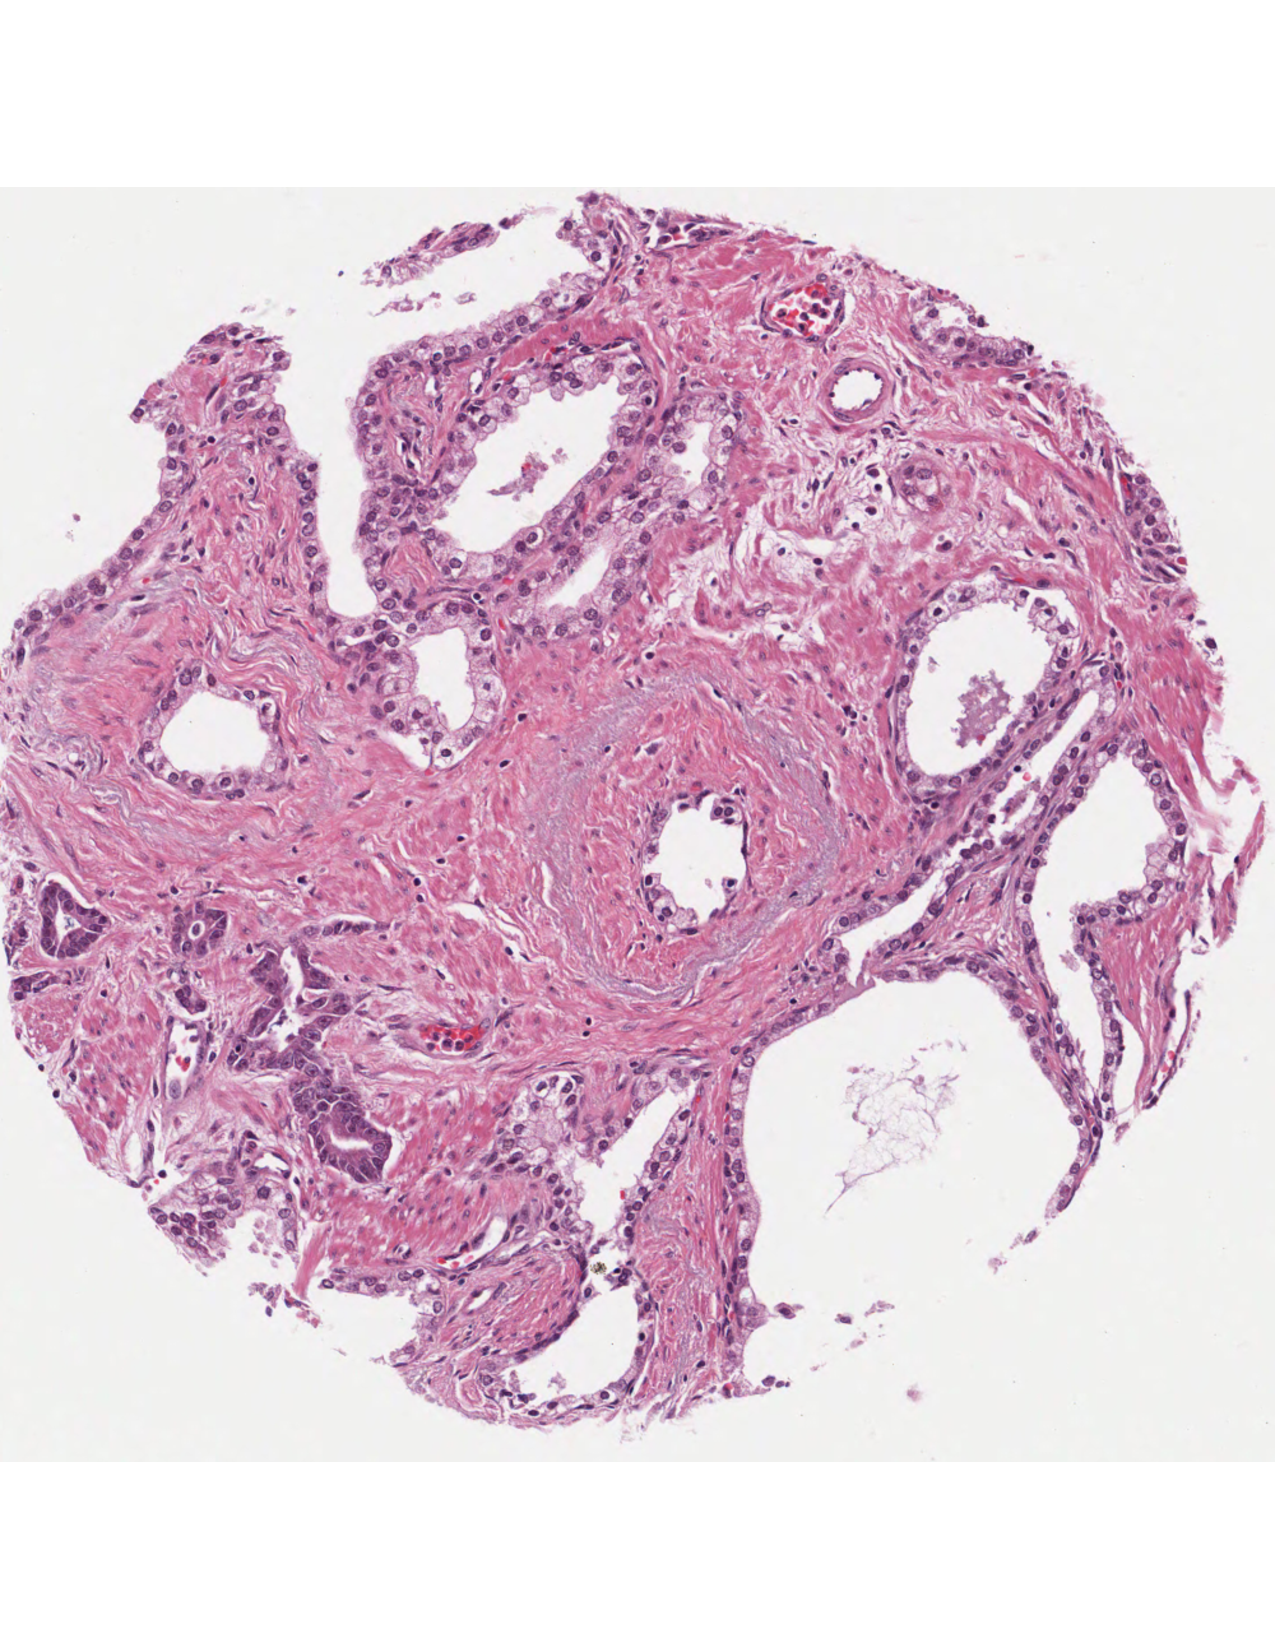
\includegraphics[width=2.0cm]{figs/108_green.pdf}
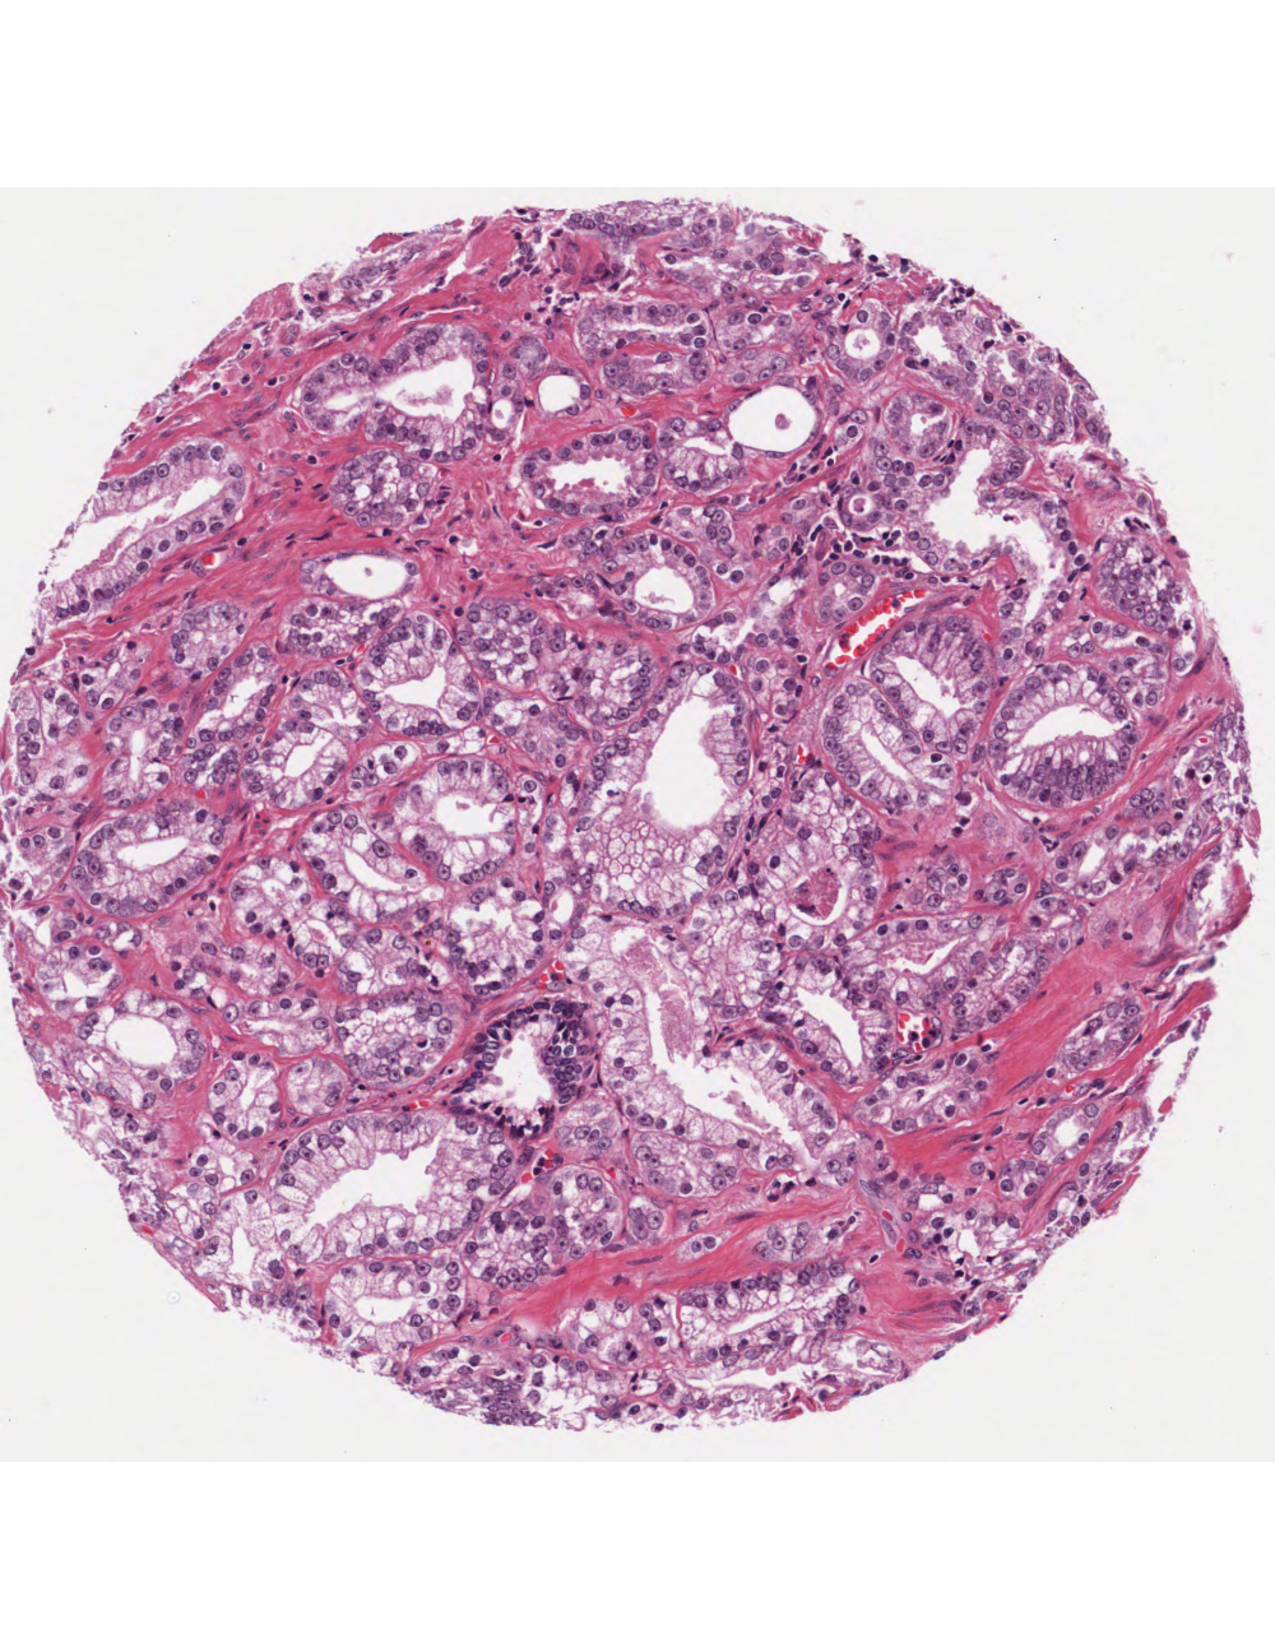
\includegraphics[width=2.0cm]{figs/109_red.pdf}
\caption{Stained tissue images in the dataset}
\label{fig:TissueImageExample}

\end{figure}  
  

The dataset has a nearly even split among the classes with 76 images belonging to `cancerous' class and remaining 73 `non-cancerous'. Another point to note over here is that the tissues in these images were stained in two separate batches, so the dataset may not be indicative of the variability in staining. Note that this dataset is significantly bigger than the datasets used in other works - indeed \cite{naik2007gland} uses a dataset of 44 images for their approach.

\subsection{Patch-Level Features}
In this section, we provide the results for the patch-level feature extraction and classification.

\subsection{Image-Level Features}
In this section, we discuss the results for the different features we extract from the images. The classifiers we try out on the extracted features are 
\begin{itemize}
\item Support Vector Machine with Gaussian Kernel (\textbf{\texttt{SVM}})
\item K-nearest neighbor classifier (\textbf{\texttt{KNN}})
\item Decision Tree classifier (\textbf{\texttt{DTREE}})
\end{itemize}
For each of these classifiers, 10-fold cross-validation was performed. 

\begin{tabular}{|c|c|c|c| }
\hline
 & \textbf{\texttt{SVM}} & \textbf{\texttt{KNN}} & \textbf{\texttt{DTREE}} \\ \hline
\textbf{\texttt{LocalMin}} & 81.2\% & 69.8\% & 71.8\% \\ \hline
\textbf{\texttt{kMeans}} &  4 & 5 & 6 \\ \hline
\textbf{ \texttt{CircleConv}} & 77.9\% & 73.2\% & 70.5\% \\ \hline
\end{tabular}

